%# -*- coding:utf-8 -*-
\documentclass[10pt,aspectratio=169,mathserif]{beamer}		
%设置为 Beamer 文档类型,设置字体为 10pt,长宽比为16:9,数学字体为 serif 风格

%%%%-----导入宏包-----%%%%
\usepackage{hit}			%导入 CCNU 模板宏包
\usepackage{ctex}			%导入 ctex 宏包,添加中文支持
\usepackage{amsmath,amsfonts,amssymb,bm}   %导入数学公式所需宏包
\usepackage{color}			 %字体颜色支持
\usepackage{graphicx,hyperref,url}
\usepackage{metalogo}	% 非必须
\usepackage{color}
%% 上文引用的包可按实际情况自行增删
%%%%%%%%%%%%%%%%%%	


\beamertemplateballitem		%设置 Beamer 主题

%%%%------------------------%%%%%
\catcode`\。=\active         %或者=13
\newcommand{。}{.}				
%将正文中的“。”号转换为“.”。中文标点国家规范建议科技文献中的句号用圆点替代
%%%%%%%%%%%%%%%%%%%%%

%%%%----首页信息设置----%%%%
\title[开关电源设计开发实践与创新思维课程报告]{开关电源设计开发实践与创新思维课程报告}
\subtitle{——交错串联电容分接Buck降压电路 \ ISC-TaB}			
%%%%----标题设置


\author[Wang.Jiang.Cao]{
  第四组:王浩瑞 \ 蒋佳诚 \ 曹广旭 }
%%%%----个人信息设置
  
\institute[IOPP]{
  电气工程及自动化学院 \\ 
  }
%%%%----机构信息

\date[Oct. 20 2020]{
  2020年10月20日}
%%%%----日期信息
  
\begin{document}

\begin{frame}
	\titlepage
\end{frame}				%生成标题页

\section{提纲}
\begin{frame}
	\frametitle{提纲}
	\tableofcontents
\end{frame}				%生成提纲页

\section{背景}
\begin{frame}
	\frametitle{背景}

	\begin{itemize}
		\item 通讯、工业系统用电需要做到高低压隔离
		      \begin{itemize}
			      \item DC/DC变换器
			      \item 如何实现高降压比?
		      \end{itemize}
		\item Buck电路及其拓扑
		      \begin{itemize}
			      \item SC-Buck
			      \item Buck-Boost
			      \item \textcolor{red}{ISC-Buck}
			            \begin{itemize}
				            \item 提出ISC-Buck拓扑结构实现48V-3.3V降压
			            \end{itemize}
		      \end{itemize}
	\end{itemize}
\end{frame}

\section{参考电路图}
\begin{frame}
	\frametitle{参考电路图}
	\begin{columns}[T] % align columns
		\begin{column}<0->{.70\textwidth}
			\begin{figure}[thpb]
				\centering
				\resizebox{1\linewidth}{!}{
					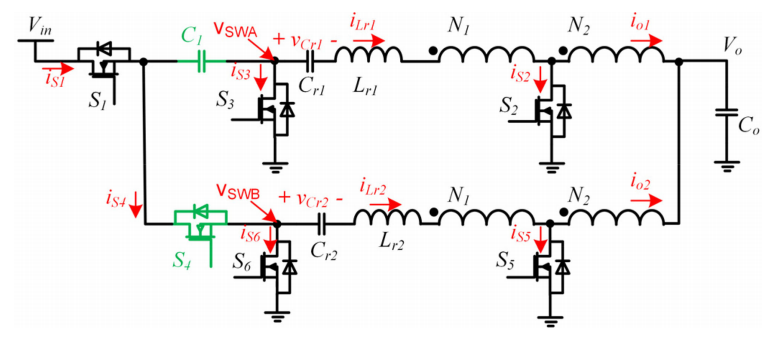
\includegraphics{figure/circuit diagram1.png}
				}
				%\includegraphics[scale=1.0]{figurefile}
				\caption{参考电路图}
				\label{fig:campus}
			\end{figure}
		\end{column}%
		\begin{column}<0->{.40\textwidth}
			\begin{itemize}
				\item 使用了六个开关管 \ MOS1-MOS6 \ \textcolor{red}{D倍降压}
				\item 电路拓扑结构具有\textcolor{red}{对称性} \ phaseA,phaseB \ \textcolor{red}{两倍降压}
				\item 使用了变压器降压 \ \textcolor{red}{n:1倍降压}
				\item  LLC软开关
			\end{itemize}
		\end{column}%
	\end{columns}
\end{frame}

\section{仿真电路图}
\begin{frame}
	\frametitle{仿真电路图}
	\begin{columns}[T] % align columns
		\begin{column}<0->{.70\textwidth}
			\begin{figure}[thpb]
				\centering
				\resizebox{1\linewidth}{!}{
					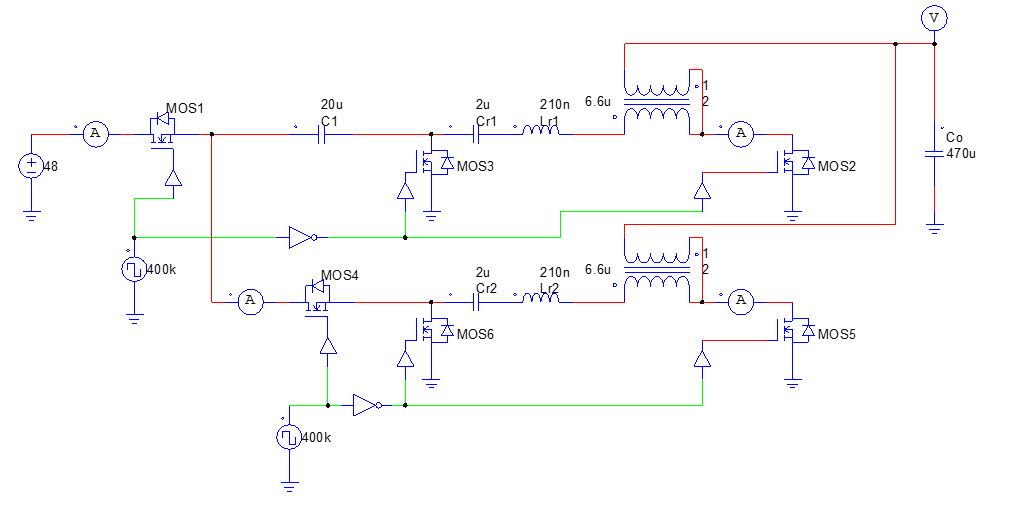
\includegraphics{figure/PSIM-circuit diagram1.png}
				}
				%\includegraphics[scale=1.0]{figurefile}
				\caption{仿真电路图}
				\label{fig:campus}
			\end{figure}
		\end{column}%
		\begin{column}<0->{.40\textwidth}
			\begin{itemize}
				\item 注意MOS1-MOS6的开关顺序和相位
				\item 注意$L_r$和$L_m$的选用
				\item 输出选用大容值电容
			\end{itemize}
		\end{column}%
	\end{columns}
\end{frame}

\begin{frame}
	\frametitle{仿真电路图}
	\begin{columns}[T] % align columns
		\begin{column}<0->{.60\textwidth}
			\begin{figure}[thpb]
				\centering
				\resizebox{1\linewidth}{!}{
					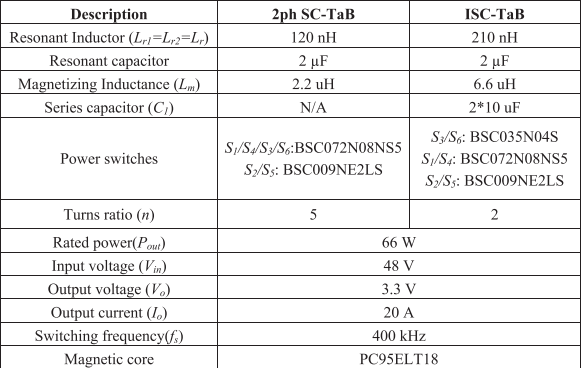
\includegraphics{figure/parameter_table figure.png}
				}
				%\includegraphics[scale=1.0]{figurefile}
				\caption{元件参数表}
				\label{fig:campus}
			\end{figure}
		\end{column}%
	\end{columns}
\end{frame}

\section{电路原理}
\begin{frame}
	\frametitle{电路原理}
	\begin{columns}[T] % align columns
		\begin{column}<0->{.30\textwidth}
			\begin{figure}[thpb]
				\centering
				\resizebox{1\linewidth}{!}{
					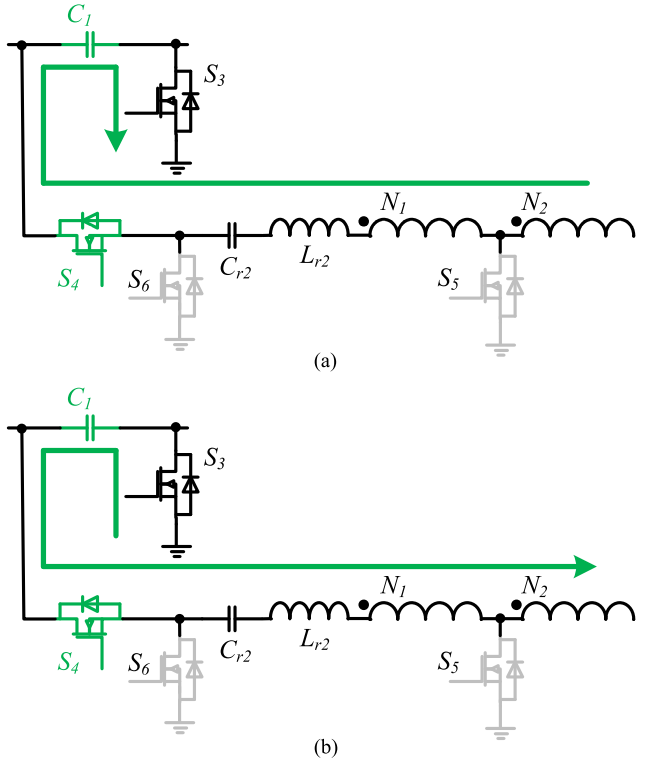
\includegraphics{figure/current actual direction in t0-t3.png}
				}
				%\includegraphics[scale=1.0]{figurefile}
				\caption{电流流向(开态)}
				\label{fig:campus}
			\end{figure}
		\end{column}%
		\begin{column}<0->{.30\textwidth}
			\begin{figure}[thpb]
				\centering
				\resizebox{1\linewidth}{!}{
					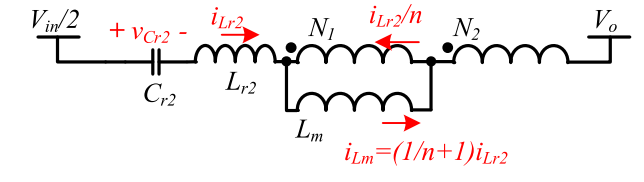
\includegraphics{figure/current value in t0-t2.png}
				}
				%\includegraphics[scale=1.0]{figurefile}
				\caption{电流大小关系(开态)}
				\label{fig:campus}
			\end{figure}
		\end{column}%
	\end{columns}
\end{frame}

\begin{frame}
	\frametitle{电路原理}
	\begin{columns}[T] % align columns
		\begin{column}<0->{.36\textwidth}
			\begin{figure}[thpb]
				\centering
				\resizebox{1\linewidth}{!}{
					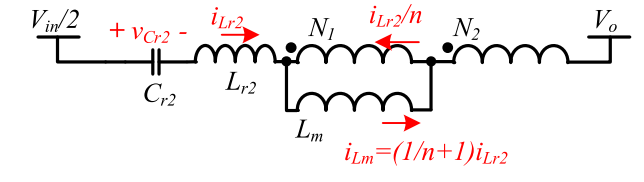
\includegraphics{figure/current value in t0-t2.png}
				}
				%\includegraphics[scale=1.0]{figurefile}
				\caption{电流大小关系(开态)}
				\label{fig:campus}
			\end{figure}
		\end{column}%
		\begin{column}<0->{.40\textwidth}
			\begin{equation}
				\left\{\begin{array}{l}
					\frac{V_{\mathrm{in}}}{2}-V_{o}-v_{\mathrm{Cr} 2}=L_{r 2} \frac{d i_{\mathrm{Lr} 2}}{d t}+L_{m} \frac{d i_{\mathrm{Lr} 2}}{d t} \frac{(n+1)^{2}}{n^{2}} \\
					i_{\mathrm{Lr} 2}=C_{r 2} \frac{d v_{\mathrm{Cr} 2}}{d t}
				\end{array}\right.
			\end{equation}
		\end{column}%
	\end{columns}
\end{frame}

\begin{frame}
	\frametitle{电路原理}
	\begin{columns}[T] % align columns
		\begin{column}<0->{.30\textwidth}
			\begin{figure}[thpb]
				\centering
				\resizebox{1\linewidth}{!}{
					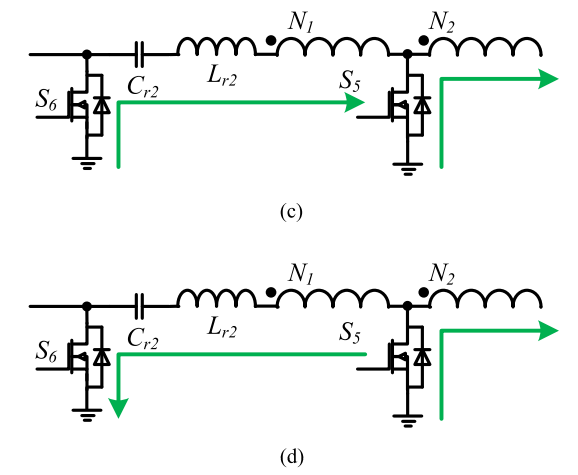
\includegraphics{figure/current actual direction in t3-t0.png}
				}
				%\includegraphics[scale=1.0]{figurefile}
				\caption{电流流向(关态)}
				\label{fig:campus}
			\end{figure}
		\end{column}%
		\begin{column}<0->{.30\textwidth}
			\begin{figure}[thpb]
				\centering
				\resizebox{1\linewidth}{!}{
					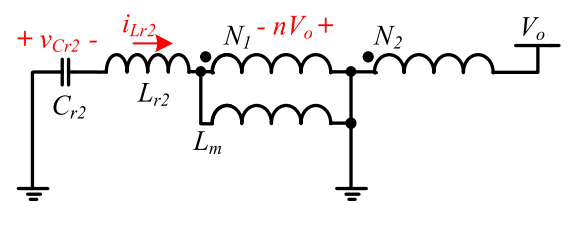
\includegraphics{figure/current value in t3-t5.png}
				}
				%\includegraphics[scale=1.0]{figurefile}
				\caption{电流大小关系(关态)}
				\label{fig:campus}
			\end{figure}
		\end{column}%
	\end{columns}
\end{frame}

\begin{frame}
	\frametitle{电路原理}
	\begin{columns}[T] % align columns
		\begin{column}<0->{.36\textwidth}
			\begin{figure}[thpb]
				\centering
				\resizebox{1\linewidth}{!}{
					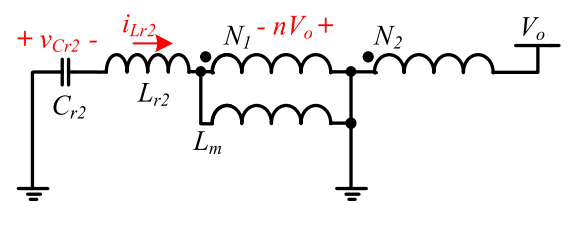
\includegraphics{figure/current value in t3-t5.png}
				}
				%\includegraphics[scale=1.0]{figurefile}
				\caption{电流大小关系(关态)}
				\label{fig:campus}
			\end{figure}
		\end{column}%
		\begin{column}<0->{.36\textwidth}
			\begin{equation}
				\left\{\begin{array}{l}
					-v_{\mathrm{Cr} 2}+n V_{o}=L_{r 2} \frac{d i_{\mathrm{Lr} 2}}{d t} \\
					i_{\mathrm{Lr} 2}=C_{r 2} \frac{d v_{\mathrm{Cr} 2}}{d t}
				\end{array}\right.
			\end{equation}
		\end{column}%
	\end{columns}
\end{frame}

\section{降压比计算}
\begin{frame}
	\frametitle{降压比计算}
	\begin{itemize}
		\item 谐振电感电压$V_{L_{r2}}$
		      \begin{equation}
			      V_{\mathrm{Lr} 2}=\frac{\frac{V_{\mathrm{in}}}{2}-V_{o}-V_{\mathrm{Cr} 2}}{1+\frac{L_{m}}{L_{r 2}} \cdot \frac{(n+1)^{2}}{n^{2}}}
		      \end{equation}
	\end{itemize}
	\begin{itemize}
		\item 变压器励磁电感电压$V_{L_{m}}$
		      \begin{equation}
			      V_{\mathrm{Lm}}=\frac{L_{m}}{L_{r 2}} \cdot\left(1+\frac{1}{n}\right) \cdot V_{\mathrm{Lr} 2}
		      \end{equation}
	\end{itemize}
	\begin{itemize}
		\item 伏秒平衡(开态)
		      \begin{equation}
			      V_{\mathrm{Lr} 2} \cdot D+\left(-V_{\mathrm{Cr} 2}+n V_{o}\right) \cdot(1-D)=0
		      \end{equation}
	\end{itemize}
	\begin{itemize}
		\item 伏秒平衡(关态)
		      \begin{equation}
			      V_{\mathrm{Lm}} \cdot D+(1-D)\left(-n V_{o}\right)=0
		      \end{equation}
	\end{itemize}
\end{frame}


\begin{frame}
	\frametitle{降压比计算}
	\begin{itemize}
		\item 降压比
	\end{itemize}
	\begin{equation}
		\frac{V_{o}}{V_{\text {in }}}=\frac{D}{2 \cdot\left(n+1+\frac{L_{r}}{L_{m}} \cdot \frac{n^{2}}{n+1}\right)}
	\end{equation}
\end{frame}

\section{结论/思考}
\begin{frame}
	\frametitle{结论/思考}
	\begin{itemize}
	\item 该电路成功实现了48V-3.3V的10倍以上降压
	\item 优点
		\begin{itemize}
			\item 单极降压比高
			\item 输出电流大,带负载能力强
		\end{itemize}
	\item 可能存在的问题
		\begin{itemize}
			\item 效率
			\begin{itemize}
				\item 解决措施:intergrate the inductor and the PCB \\
				开关电源的EMC设计 \url{https://zhuanlan.zhihu.com/p/90704119}
			\end{itemize}
			\item 结构复杂程度
		\end{itemize}
	\end{itemize}
\end{frame}

\section{参考文献}
\begin{frame}{参考文献}
	\begin{thebibliography}{99}
		\bibitem{zhao1} Lanhua~Zhang,Sombuddha~Chakraborty {\sl An \ Interleaved \ Series-Capacitor \ Tapped \ Buck \ Converter \ for \ High
		Step-Down \ DC/DC \ Application}, VOL.34,JULY,2019,IEEE \ TRANSACTIONS \ ON \ POWER ELECTRONICS

	\end{thebibliography}
\end{frame}




\end{document}